\documentclass[tikz,border=8pt]{standalone}
\usepackage[dvipsnames]{xcolor}
\usetikzlibrary{shapes.geometric,arrows.meta,positioning,fit,backgrounds,calc}

\begin{document}
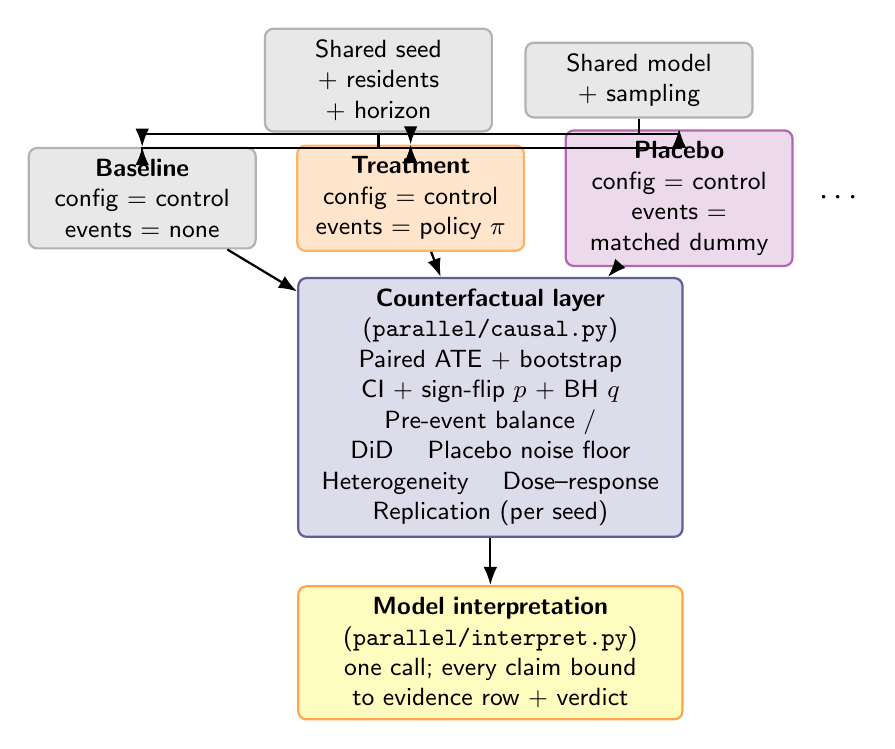
\begin{tikzpicture}[
  font=\sffamily\small,
  wbox/.style={rectangle, draw, thick, rounded corners=3pt, align=center, minimum height=0.9cm, inner sep=4pt},
  world/.style={wbox, fill=OliveGreen!15, draw=OliveGreen!70, text width=2.6cm},
  base/.style={wbox, fill=gray!18, draw=gray!60, text width=2.6cm},
  treat/.style={wbox, fill=orange!20, draw=orange!60, text width=2.6cm},
  plac/.style={wbox, fill=Purple!15, draw=Purple!60, text width=2.6cm},
  infbox/.style={wbox, fill=MidnightBlue!15, draw=MidnightBlue!70, text width=4.6cm},
  interp/.style={wbox, fill=yellow!25, draw=orange!70, text width=4.6cm},
  ar/.style={-Latex, thick},
  >={Stealth[length=2.5mm]}
]

% Top: shared inputs
\node[base] (seed) at (0, 1.5) {Shared seed + residents + horizon};
\node[base, right=0.4cm of seed] (model) {Shared model + sampling};

% Worlds (3 visible; "..." indicates up to 8)
\node[base] (w0) at (-3.0, 0) {%
  \textbf{Baseline}\\
  config = control\\
  events = none};
\node[treat, right=0.5cm of w0] (w1) {%
  \textbf{Treatment}\\
  config = control\\
  events = policy $\pi$};
\node[plac, right=0.5cm of w1] (wp) {%
  \textbf{Placebo}\\
  config = control\\
  events = matched dummy};
\node[font=\large, right=0.2cm of wp] (etc) {$\cdots$};

% Inference
\node[infbox, below=1.0cm of $(w0)!0.5!(etc)$] (inf) {%
  \textbf{Counterfactual layer} (\texttt{parallel/causal.py})\\
  Paired ATE + bootstrap CI + sign-flip $p$ + BH $q$\\
  Pre-event balance / DiD \quad Placebo noise floor\\
  Heterogeneity \quad Dose--response \quad Replication (per seed)};

% Interpretation (optional)
\node[interp, below=0.6cm of inf] (itp) {%
  \textbf{Model interpretation} (\texttt{parallel/interpret.py})\\
  one call; every claim bound to evidence row + verdict};

% Arrows
\draw[ar] (seed.south) -- ++(0,-0.2) -| (w0.north);
\draw[ar] (seed.south) -- ++(0,-0.2) -| (w1.north);
\draw[ar] (seed.south) -- ++(0,-0.2) -| (wp.north);
\draw[ar] (model.south) -- ++(0,-0.2) -| (w0.north);
\draw[ar] (model.south) -- ++(0,-0.2) -| (w1.north);
\draw[ar] (model.south) -- ++(0,-0.2) -| (wp.north);
\draw[ar] (w0) -- (inf);
\draw[ar] (w1) -- (inf);
\draw[ar] (wp) -- (inf);
\draw[ar] (inf) -- (itp);

\end{tikzpicture}
\end{document}
